\documentclass[xcolor=svgnames]{beamer}
\mode<presentation>
{
      \setbeamertemplate{footline}[page number]
      \setbeamercovered{transparent}
      \setbeamertemplate{navigation symbols}{}
      \usecolortheme[named=DarkGreen]{structure}
}

\usepackage[english]{babel}
\usepackage{times}
\usepackage{url}
\usepackage{CJKutf8}
\usepackage{graphics}
\usepackage{amsmath}

\begin{document}
\begin{CJK*}{UTF8}{gbsn}


\title{文件系统}

\begin{frame}
\maketitle
\end{frame}


\begin{frame}{操作系统中三个最重要的概念}
\begin{enumerate}
\item 把处理器CPU抽象为\alert{进程}
\item[]
\item 把物理内存抽象为(虚拟)\alert{地址空间}
\item[]
\item 把永久存储介质(如硬盘)抽象为\alert{文件}
\end{enumerate}
\end{frame}


\begin{frame}{文件的类型}
\begin{enumerate}
\item 普通文件(.doc, .c, .cpp, .pdf, .exe)
\item[]
\item 目录
\item[]
\item 字符设备文件(第5章)
\item[]
\item 块设备文件(第5章)
\end{enumerate}
\end{frame}

\begin{frame}{文件的存取方法}
\begin{enumerate}
\item 顺序存取(sequential access): 只能按前后顺序访问每个字节,不能随机访问。例如磁带上的文件系统
\item[]
\item 随机存取(random access): 可以按照任意顺序访问文件的各个字节,例如磁盘文件系统
\item[]
\end{enumerate}
\end{frame}

\begin{frame}{文件的属性}
\begin{itemize}
\item protection
\item password
\item creator
\item owner
\item read-only flag
\item lock flag
\item creation time
\item time of last access
\item current size
\end{itemize}
\end{frame}

\begin{frame}{针对文件的操作}
\begin{itemize}
\item create
\item delete
\item open
\item close
\item read
\item write
\item append
\item seek (仅限可随机访问的文件)
\item get attributes 
\item set attributes
\item rename
\end{itemize}
\end{frame}

\begin{frame}{针对目录的操作}
\begin{itemize}
\item create
\item delete
\item opendir
\item closedir
\item readdir
\item rename
\item link (图示及命令ln)
\item unlink (图示, 命令?)
\end{itemize}
\end{frame}

\begin{frame}{文件的实现}
\alert{核心问题}是记录每个文件在存储介质(如磁盘)上存放的位置。
\end{frame}

\begin{frame}{文件的实现: 连续存储方式}
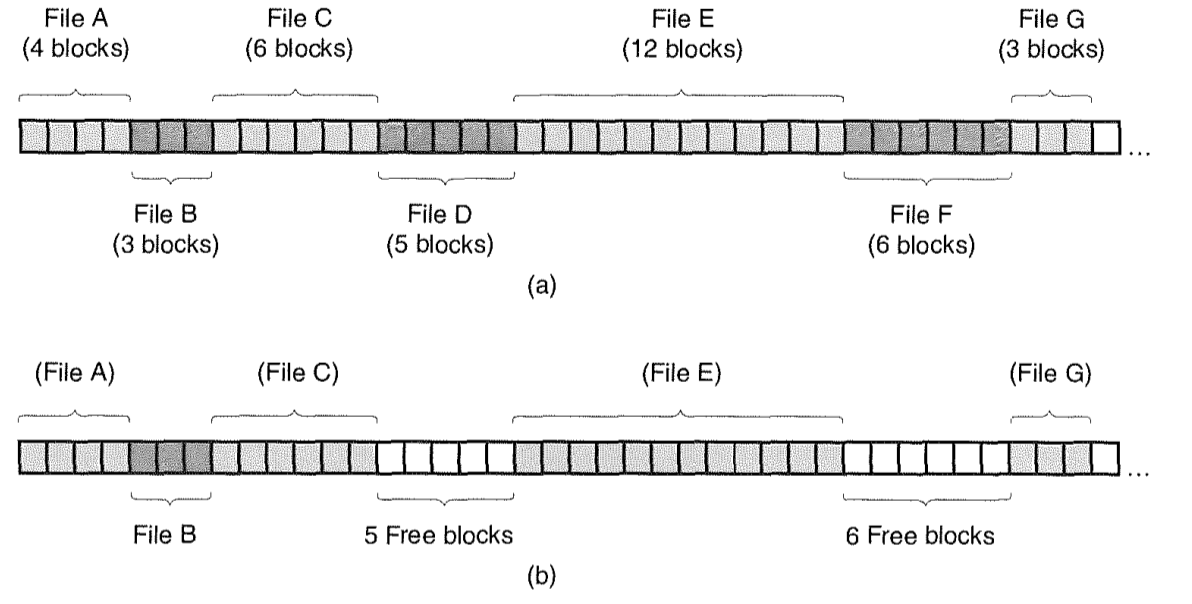
\includegraphics[width=1.0\textwidth]{cont.png}
\end{frame}

\begin{frame}{文件的实现: 连续存储方式}
%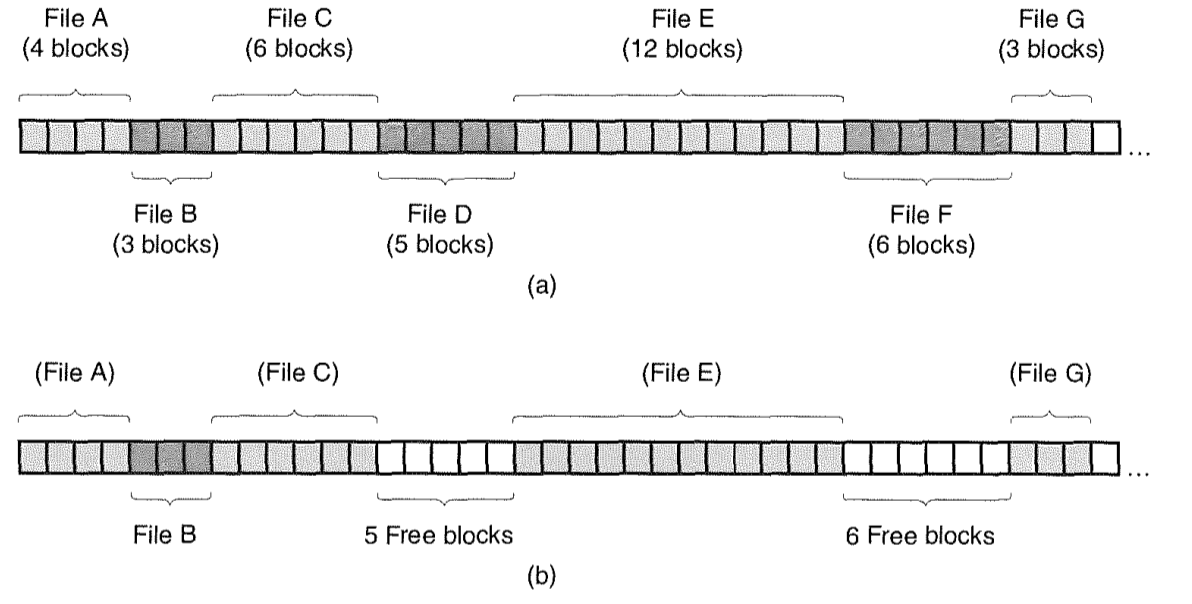
\includegraphics[width=1.0\textwidth]{cont.png}
连续存储方式有两个重要优点:
\begin{itemize}
\item 实现容易:只需记录每个文件在磁盘上起始块地址,以及所占的总块数
\item 读写速度非常块:每次读写仅需1次机械移动寻址过程
\end{itemize}

\alert{缺点?} --- 容易导致文件系统大量碎片(前图)

\alert{应用?} --- CD-ROM上的文件系统, why?
\end{frame}

\begin{frame}{文件的实现: 线性链表存储方式}
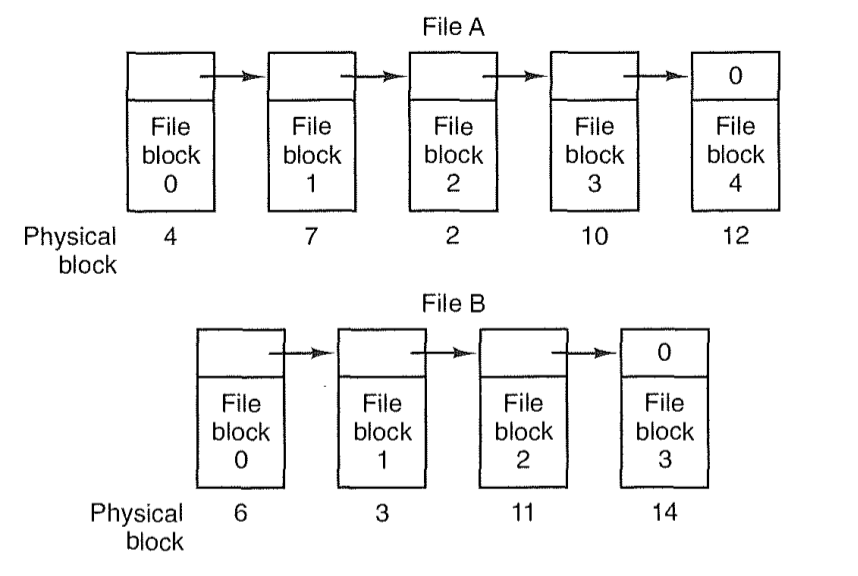
\includegraphics[width=1.0\textwidth]{linked.png}

\alert{注}: 每个磁盘块的前几个字节用于记录存储该文件的下一个磁盘块地址
\end{frame}

\begin{frame}{文件的实现: 线性链表存储方式}
线性链表存储方式的优点:
\begin{itemize}
\item 只需记录每个文件在磁盘上的起始地址
\item 避免碎片问题
\end{itemize}

缺点:不利于随机访问, why?
\end{frame}

\begin{frame}{文件的实现: I-nodes}
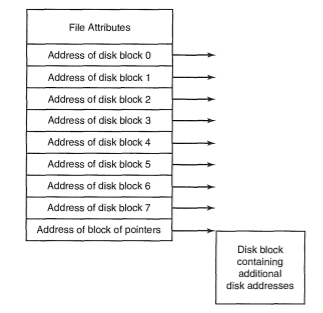
\includegraphics[width=0.8\textwidth]{inodes.png}
\end{frame}

\begin{frame}{文件的实现: I-nodes}
结合命令ln以及ls -li理解i-node实现方法

目录的实现方法?
\end{frame}

\begin{frame}{文件系统的布局}
%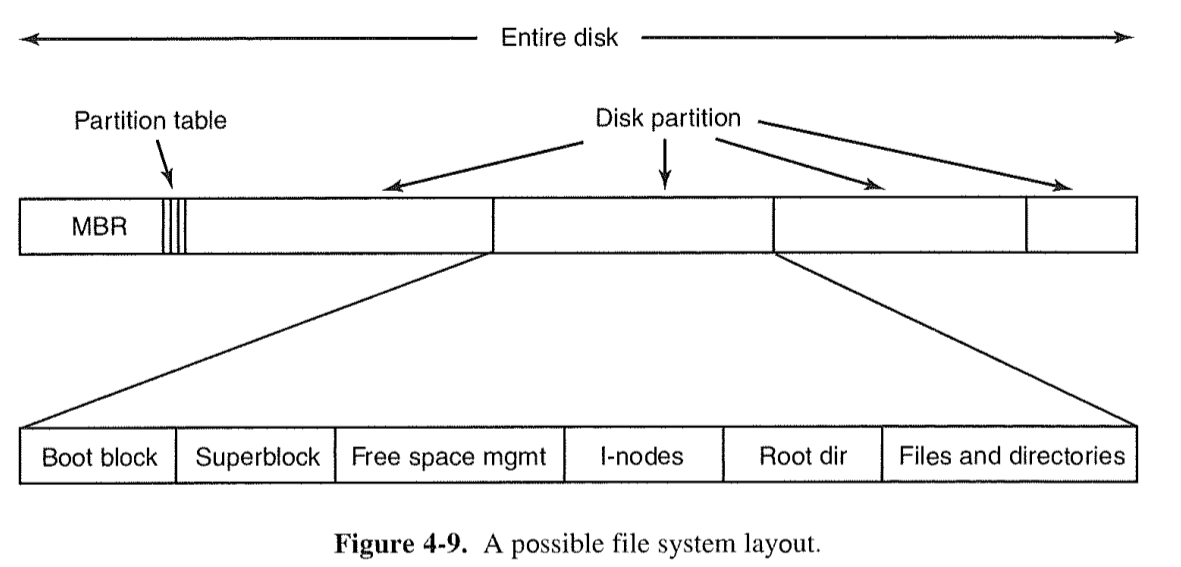
\includegraphics[width=1.0\textwidth]{layout.png}
考虑磁盘上的文件系统:
\begin{itemize}
\item 磁盘可以进行分区,用磁盘分区表记录每个分区的边界
\item 第0扇区:MBR(Master Boot Record, 主引导记录), 存放引导程序及磁盘分区表
\item MBR中的引导程序选择某个分区中的操作系统进行引导
\item 每个分区中有一个磁盘块用于启动该分区上的操作系统(boot block)
\item 超级块(superblock): 存放该分区上的文件系统参数(类型、块数等信息)
\end{itemize}
\end{frame}

\begin{frame}{文件系统的布局}
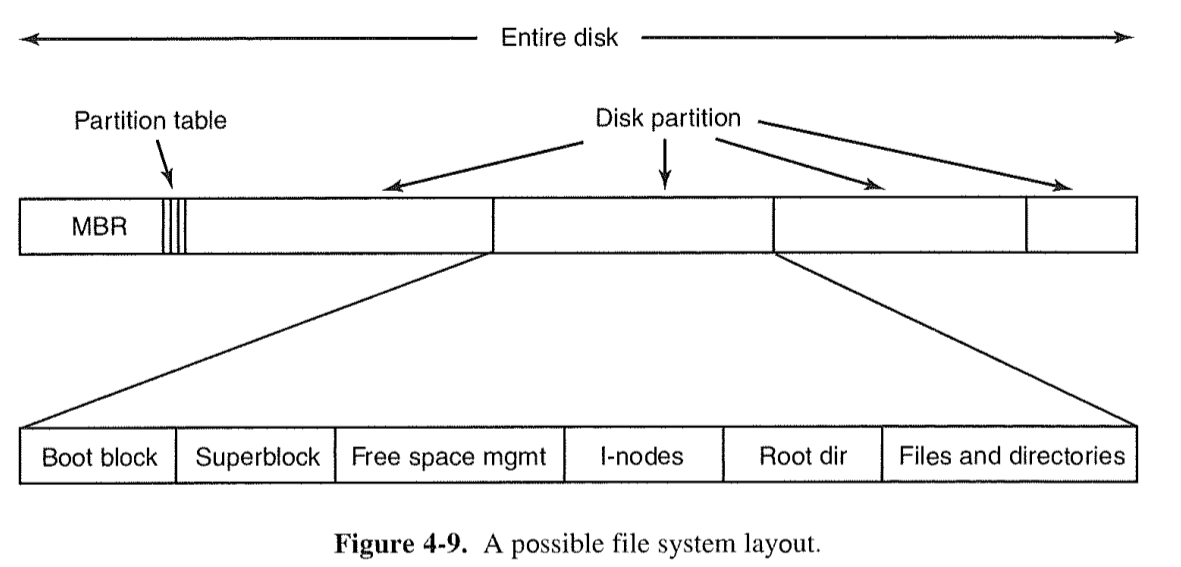
\includegraphics[width=1.0\textwidth]{layout.png}
\end{frame}

%\begin{frame}{对临界资源的互斥访问}
%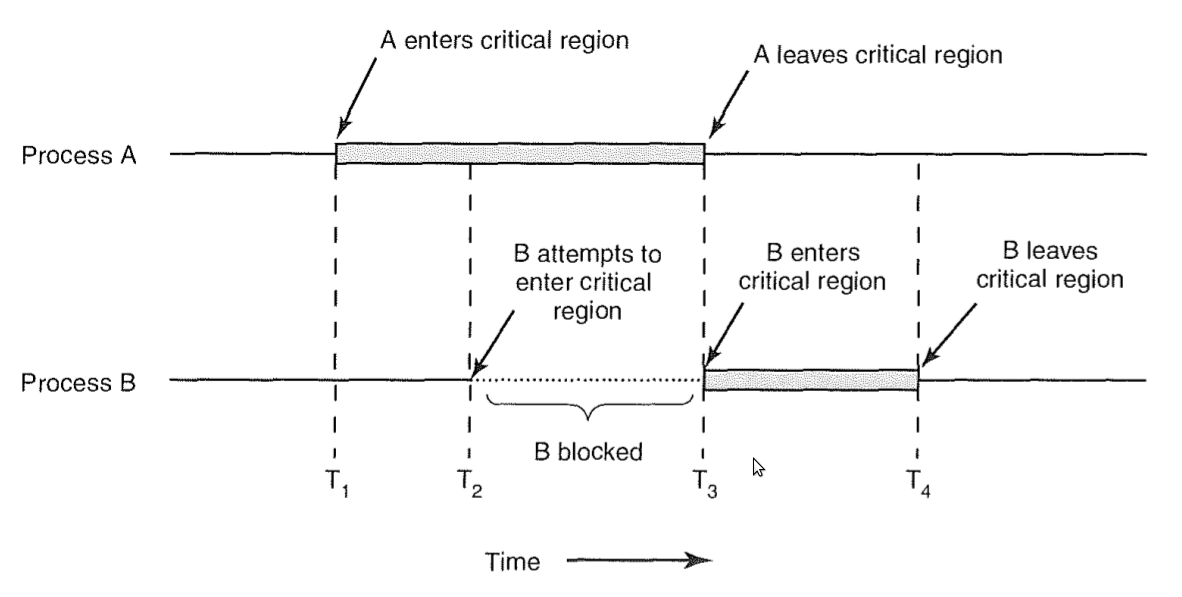
\includegraphics[width=1.0\textwidth]{mutual.png}
%\end{frame}

%\begin{frame}{用信号量解决生产者--消费者问题}
%\begin{columns}[b]
%\column{.5\textwidth}
%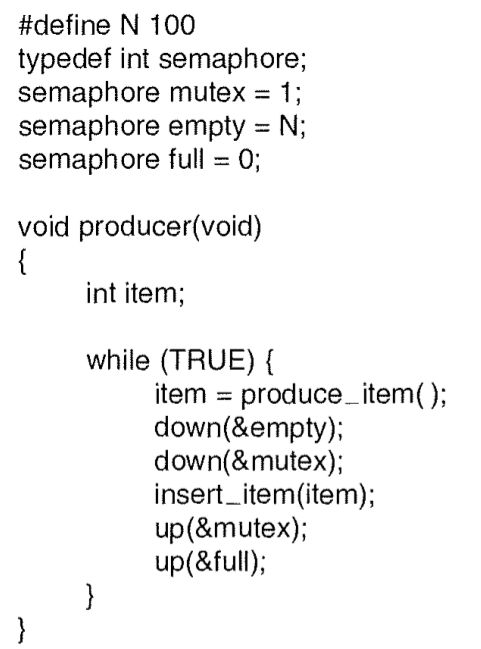
\includegraphics[width=1.0\textwidth]{prodsem.png}
%\column{.5\textwidth}
%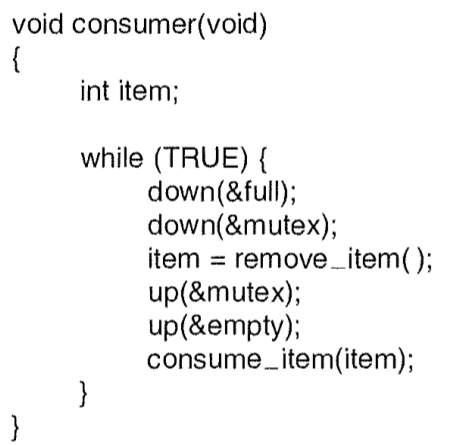
\includegraphics[width=1.0\textwidth]{conssem.png}
%\end{columns}%[t]

%该方案中,信号量empty和full具有计数和同步功能,而mutex仅有互斥功能。
%\end{frame}

%\begin{frame}{专门用来实现互斥的特殊信号量 -- 互斥锁}
%互斥锁只有两种状态:locked (1) / unlocked (0)
%
%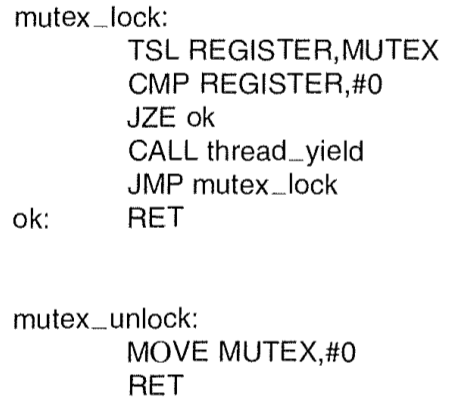
\includegraphics[width=0.5\textwidth]{mutex.png}
%\end{frame}

%\begin{frame}{互斥锁与忙等待的区别}
%\begin{columns}[b]
%\column{.5\textwidth}
%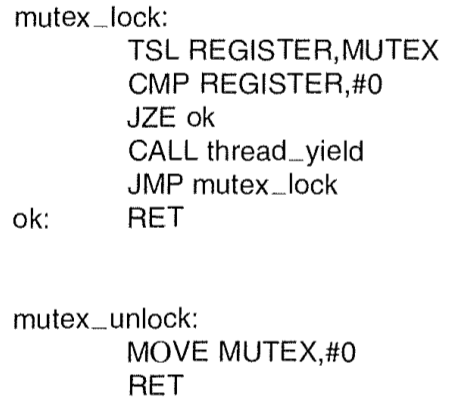
\includegraphics[width=1.0\textwidth]{mutex.png}
%\column{.5\textwidth}
%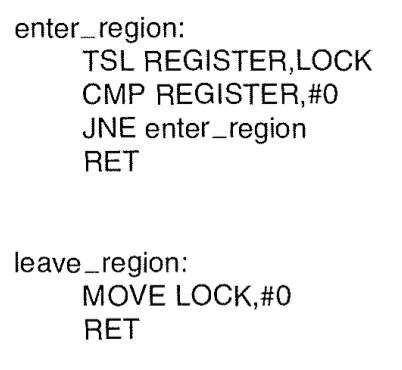
\includegraphics[width=1.0\textwidth]{tsl.png}
%\end{columns}%[t]
%后者:不断利用CPU指令测试临界资源,直至时间片用光被从CPU上撤下来
%\end{frame}
%
%\begin{frame}{信号量的危险情形 --- 管程机制的引入}
%\begin{columns}[b]
%\column{.5\textwidth}
%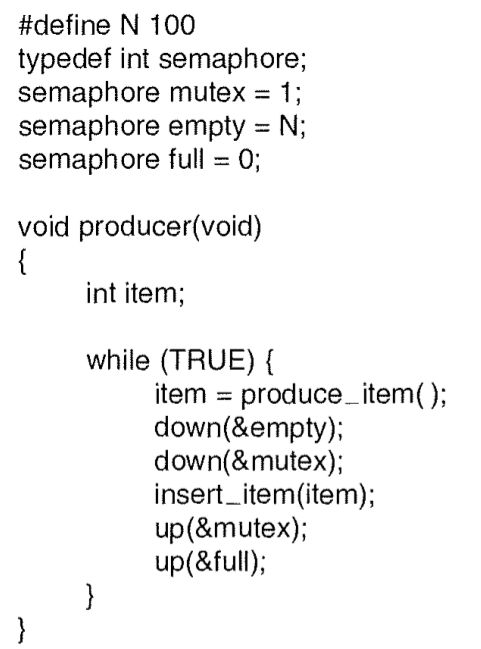
\includegraphics[width=1.0\textwidth]{prodsem.png}
%\column{.5\textwidth}
%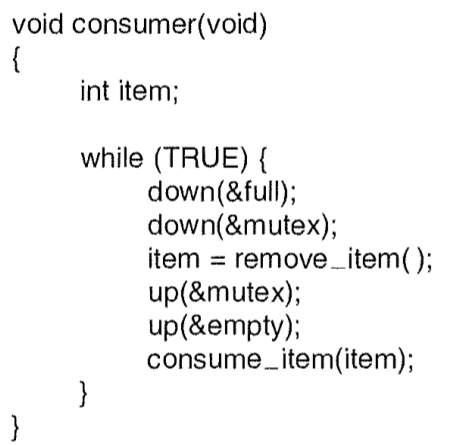
\includegraphics[width=1.0\textwidth]{conssem.png}
%\end{columns}%[t]
%\alert{危险:}如果程序员不小心把producer中的down(empty)和down(mutex)顺序颠倒,
%则当缓冲区满时,会发生什么?
%\end{frame}

%\begin{frame}{信号量的危险情形 --- 管程机制的引入}
%\begin{itemize}
%\item 发生死锁。
%\item[]
%\item 因此,最好由编译器自动处理这种容易出错的程序段。---引入管程。
%\item[]
%\item 对比:C++中构造函数与析构函数
%\end{itemize}
%\end{frame}

%\begin{frame}{管程:解决生产者--消费者问题}
%\begin{columns}[b]
%\column{.5\textwidth}
%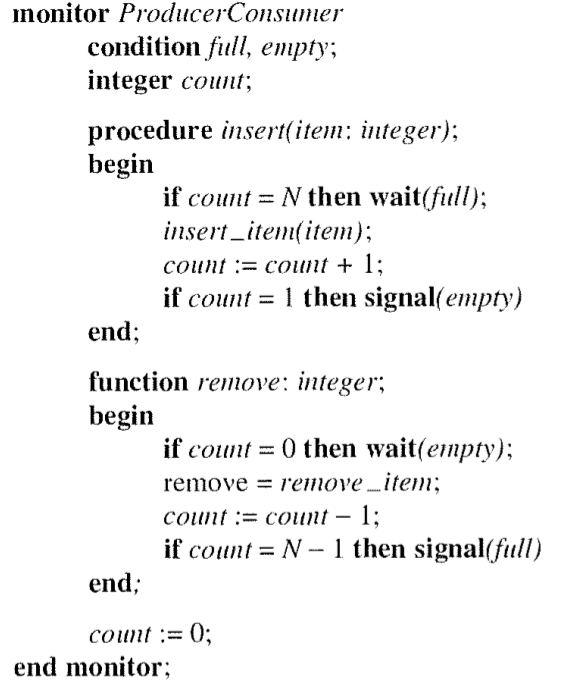
\includegraphics[width=1.0\textwidth]{mon1.png}
%\column{.5\textwidth}
%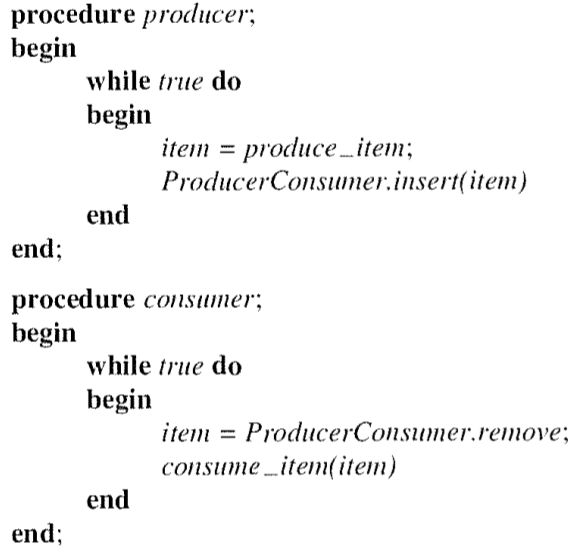
\includegraphics[width=1.0\textwidth]{mon2.png}
%\end{columns}%[t]
%
%\alert{注意概念:} 条件变量empty, full以及wait, signal
%
%此外,insert与remove之间的互斥由编译器完成
%\end{frame}

%\begin{frame}{管程:解决生产者--消费者问题}
%\begin{itemize}
%\item 管程内程序段之间的互斥(自动)
%\item 进程同步问题?:条件变量及wait, signal实现
%\begin{itemize}
%\item wait: 将当前进程阻塞,并允许其他进程进入管程
%\item signal: 将被相应条件变量阻塞的进程唤醒
%%\end{itemize}
%\item 上述方法中,signal必须是最后一条指令,为什么? 
%\end{itemize}
%\end{frame}

%\begin{frame}{消息传递机制:解决不同机器上进程间同步问题}
%\begin{columns}[b]
%\column{.5\textwidth}
%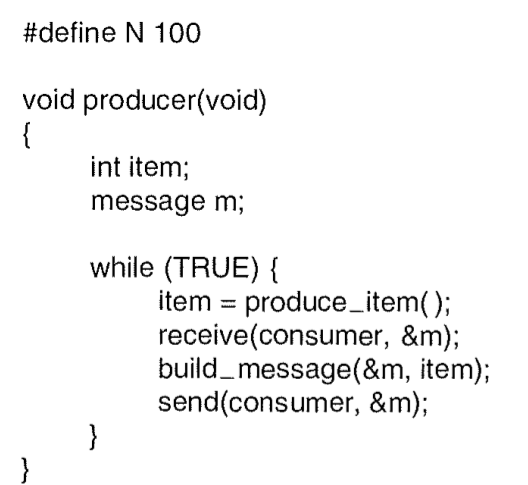
\includegraphics[width=1.0\textwidth]{msgprod.png}
%\column{.5\textwidth}
%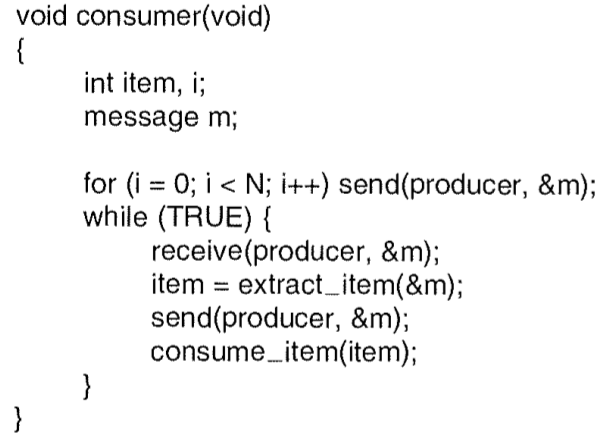
\includegraphics[width=1.0\textwidth]{msgcons.png}
%\end{columns}%[t]
%\end{frame}


\end{CJK*}
\end{document}
